ในการพัฒนาโมเดลปัญญาประดิษฐ์สำหรับจำแนกการกระทำของมนุษย์นั้นมีพื้นฐานมาจากการจำแนกวัตถุ (object classification)
หมายถึงการใช้รูปภาพหนึ่งรูปในการประมวลผลและทำนายออกมาว่าภายในรูปนั้นมีบริบทการกระทำอย่างไร โดยไม่ได้คำนึงถึงข้อมูลเชิงต่อเนื่อง (spatio-temporal information)
จากบทความ "Quo Vadis, Action Recognition? A New Model and the Kinetics Dataset"\textsuperscript{\cite{I3D}} นั้นได้พัฒนาโครงสร้างของโมเดลปัญญาประดิษฐ์ (architecture) 
ที่มีประสิทธิภาพในการประมวลผลภาพเคลื่อนไหวได้ชื่อว่า I3D หรือ inflated 3D convolution network
โดยโครงสร้างพื้นฐานของ I3D นั้นมาจาก Inception-v1\textsuperscript{\cite{Inception}} ที่ถูกพัฒนาโดย Goggle ซึ่งเป็นโครงสร้างที่มีประสิทธิภาพสูงในการจำแนกวัตถุในรูปภาพ
แล้ว I3D นั้นได้ทำการขยายมิติของโครงสร้างจาก 2 มิติ เป็น 3 มิติ เพื่อให้โมเดลปัญญาประดิษฐ์สามารถเรียนรู้ข้อมูลเชิงต่อเนื่องได้
\begin{figure}[!ht]
    \centering
    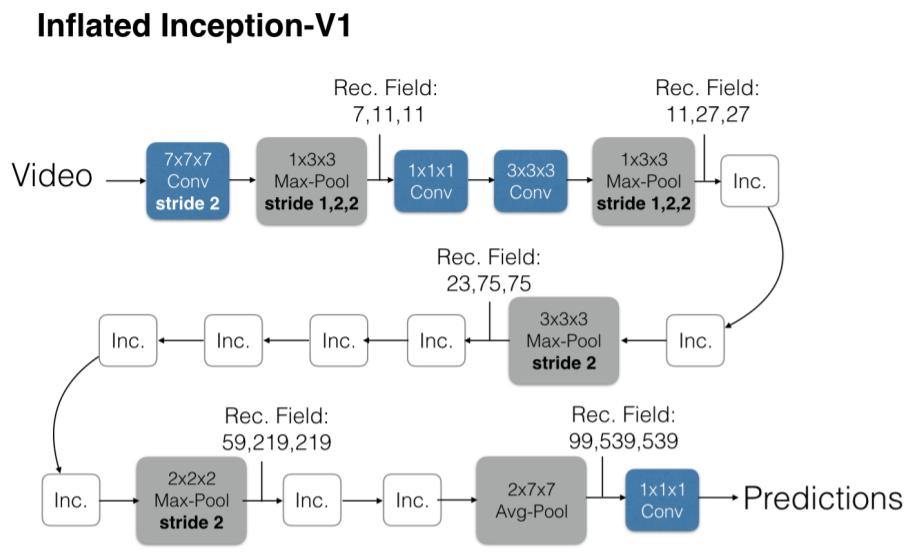
\includegraphics[width=1.0\textwidth]{chapter2/images/I3D.png}
    \caption{โครงสร้างของโมเดลปัญญาประดิษฐ์ I3D\textsuperscript{\cite{I3D}}}
    \label{fig:I3DArch}
\end{figure}

\begin{figure}[!ht]
    \centering
    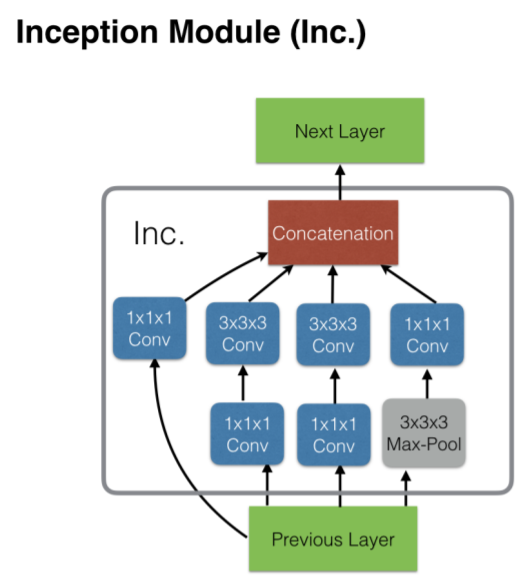
\includegraphics[width=0.7\textwidth]{chapter2/images/inceptionModule.png}
    \caption{โครงสร้างของโมเดลปัญญาประดิษฐ์ I3D\textsuperscript{\cite{I3D}}}
    \label{fig:I3DArch}
\end{figure}
% ตารางที่ \ref{tab:I3DPerformance}
